\documentclass[11pt,a4paper]{article}

% Image mode: pdf.
% Image paths stay relative. In PDF mode, place same-basename PDF conversions
% of the chapter SVG files in the assets/ directory beside this source.

\usepackage{iftex}
\ifPDFTeX
  \PackageError{handout}{This template requires XeTeX or Tectonic}{Compile with xelatex or tectonic.}
\fi

\usepackage[a4paper,top=18mm,bottom=20mm,left=20mm,right=20mm,headsep=6mm]{geometry}
\usepackage{fontspec}
\usepackage{xeCJK}
\usepackage{amsmath}
\usepackage{unicode-math}

% Font settings are intentionally visible in the generated .tex file.
% These defaults target the macOS machine used for the released PDF.
% Change the family names when compiling on another system.
\setmainfont{Songti TC}
\setsansfont{Heiti TC}
\setmonofont{Menlo}
\setCJKmainfont{Songti TC}
\setCJKsansfont{Heiti TC}
\setCJKmonofont{Heiti TC}
\setmathfont{STIX Two Math}
\XeTeXlinebreaklocale "zh"
\XeTeXlinebreakskip=0pt plus 1pt

\usepackage{xcolor}
\definecolor{HandoutBlue}{HTML}{215A91}
\definecolor{HandoutBlueLight}{HTML}{EEF5FC}
\definecolor{HandoutGreen}{HTML}{39715A}
\definecolor{HandoutGreenLight}{HTML}{EFF8F3}
\definecolor{HandoutGold}{HTML}{8A641C}
\definecolor{HandoutGoldLight}{HTML}{FFF8E8}
\definecolor{HandoutInk}{HTML}{253142}
\definecolor{HandoutMuted}{HTML}{667085}

\usepackage{graphicx}
\makeatletter
% Pandoc 3 emits an accessibility `alt` key for raster/PDF images. Older
% graphicx releases do not know that key, so accept it without changing layout.
\@ifundefined{KV@Gin@alt}{\define@key{Gin}{alt}{}}{}
\newsavebox\pandoc@box
\newcommand*\pandocbounded[1]{%
  \sbox\pandoc@box{#1}%
  \Gscale@div\@tempa{\textheight}{\dimexpr\ht\pandoc@box+\dp\pandoc@box\relax}%
  \Gscale@div\@tempb{\linewidth}{\wd\pandoc@box}%
  \ifdim\@tempb\p@<\@tempa\p@\let\@tempa\@tempb\fi
  \ifdim\@tempa\p@<\p@\scalebox{\@tempa}{\usebox\pandoc@box}%
  \else\usebox{\pandoc@box}%
  \fi
}
\makeatother
\usepackage{float}
\floatplacement{figure}{H}
% Pandoc uses LTcaptype=none for uncaptioned longtables. The caption package
% expects that name to exist as a counter even though it is never displayed.
\newcounter{none}
\usepackage{caption}
\captionsetup[figure]{labelformat=empty,labelsep=none,font=small}

\usepackage{booktabs,longtable,array,calc}
\usepackage{etoolbox}
\makeatletter
\patchcmd\longtable{\par}{\if@noskipsec\mbox{}\fi\par}{}{}
\makeatother

\usepackage[most]{tcolorbox}
\tcbuselibrary{breakable,skins}
\newtcolorbox{HandoutLearningMap}{
  enhanced,breakable,colback=HandoutBlueLight,colframe=HandoutBlue,
  boxrule=0.8pt,arc=1.5mm,left=3mm,right=3mm,top=2mm,bottom=2mm,
  before skip=8pt,after skip=10pt
}
\newtcolorbox{HandoutWorkedExample}{
  enhanced,breakable,colback=HandoutGreenLight,colframe=HandoutGreen,
  boxrule=0.65pt,arc=1.5mm,left=3mm,right=3mm,top=2mm,bottom=2mm,
  before skip=8pt,after skip=10pt
}
\newtcolorbox{HandoutSelfCheck}{
  enhanced,breakable,colback=HandoutGoldLight,colframe=HandoutGold,
  boxrule=0.65pt,arc=1.5mm,left=3mm,right=3mm,top=2mm,bottom=2mm,
  before skip=8pt,after skip=10pt
}

\usepackage{titlesec}
\titleformat{\section}{\sffamily\bfseries\Large\color{HandoutBlue}}{}{0pt}{}
\titleformat{\subsection}{\sffamily\bfseries\large\color{HandoutInk}}{}{0pt}{}
\titleformat{\subsubsection}{\sffamily\bfseries\normalsize\color{HandoutInk}}{}{0pt}{}
\titlespacing*{\section}{0pt}{1.4em}{0.55em}
\titlespacing*{\subsection}{0pt}{1.15em}{0.45em}
\titlespacing*{\subsubsection}{0pt}{0.9em}{0.35em}
\setcounter{secnumdepth}{-\maxdimen}

\usepackage{hyperref}
\usepackage{bookmark}
\IfFileExists{xurl.sty}{\usepackage{xurl}}{}
\urlstyle{same}
\hypersetup{
  colorlinks=true,
  linkcolor=HandoutBlue,
  urlcolor=HandoutBlue,
  citecolor=HandoutBlue,
  pdftitle={數2-2 數據分析},
  pdfsubject={數學},
  pdfcreator={Pandoc with the HighSchooContent LaTeX template}
}

\setlength{\parindent}{0pt}
\setlength{\parskip}{0.55em plus 0.15em minus 0.1em}
\setlength{\emergencystretch}{3em}
\setlength{\LTpre}{0.5em}
\setlength{\LTpost}{0.5em}
\renewcommand{\arraystretch}{1.18}
\providecommand{\tightlist}{%
  \setlength{\itemsep}{0pt}\setlength{\parskip}{0pt}}
\pagestyle{plain}


\begin{document}

\begin{tcolorbox}[
  enhanced,colback=white,colframe=HandoutBlue,boxrule=1.1pt,arc=2mm,
  borderline west={3pt}{0pt}{HandoutBlue},left=5mm,right=4mm,top=4mm,bottom=4mm
]
{\sffamily\small\bfseries\color{HandoutBlue}學生講義}\par
{\sffamily\bfseries\LARGE\color{HandoutInk}數2-2 數據分析}\par
\vspace{0.35em}{\large 用中心、分散、標準化與線性模型，從資料回答可比較的問題}\par
\vspace{0.45em}{\small\color{HandoutMuted}%
科目：數學
\quad 課程：普通高中數學 第二冊
\quad 版本：學生版｜核心＋理解
\quad 校訂：2026-08-29
}\par
\vspace{0.25em}{\small\color{HandoutMuted}範圍：114 學年度數學第二冊第 2 章；一維數據、百分位數、標準差、標準化、散布圖、相關係數與最小平方直線}\par
\end{tcolorbox}


\begin{HandoutLearningMap}

\subsection{本章問題與能力}\label{ux672cux7ae0ux554fux984cux8207ux80fdux529b}

\begin{enumerate}
\def\labelenumi{\arabic{enumi}.}
\tightlist
\item
  一群資料的中心應如何用算術平均、加權平均或幾何平均描述？
\item
  百分位數、四分位數、四分位距與標準差各保留了哪些資訊？
\item
  資料經過伸縮與平移後，平均數、標準差及標準化數據如何改變？
\item
  散布圖與相關係數如何描述兩個變量的線性關係？
\item
  最小平方直線如何從資料建立預測模型，殘差又如何呈現模型誤差？
\end{enumerate}

本章路徑：中心位置 → 排序位置 → 分散程度 → 標準化 → 線性相關 → 線性預測。

\end{HandoutLearningMap}

\section{0. 本章實際用途：把大量觀測整理成可比較的資訊}\label{ux672cux7ae0ux5be6ux969bux7528ux9014ux628aux5927ux91cfux89c0ux6e2cux6574ux7406ux6210ux53efux6bd4ux8f03ux7684ux8cc7ux8a0a}

一組原始數據常同時包含三種資訊：典型值落在哪裡、個體差異有多大，以及變量之間是否共同改變。平均數描述平衡位置，百分位數描述排序位置，標準差描述資料到平均數的典型距離。三者回答的問題不同，因此報告資料時通常要配合使用。

標準化把「高於平均多少」換成「高於平均幾個標準差」。不同科目的考試、不同單位的測量或不同族群的紀錄，便能放到共同尺度比較。醫療檢驗、品質管理與運動表現分析都會使用這個轉換。

兩個變量成對出現時，散布圖先顯示資料形狀，相關係數再濃縮線性方向與緊密程度。若散布點大致沿直線排列，最小平方法可建立預測式；預測仍需限制在資料涵蓋的情境與範圍內，並配合殘差判斷模型是否合適。

\section{1. 資料的中心：算術、加權與幾何平均}\label{ux8cc7ux6599ux7684ux4e2dux5fc3ux7b97ux8853ux52a0ux6b0aux8207ux5e7eux4f55ux5e73ux5747}

\subsection{1.1 算術平均數與平衡性質}\label{ux7b97ux8853ux5e73ux5747ux6578ux8207ux5e73ux8861ux6027ux8cea}

一維數據只有一個觀測變量，例如一班學生的身高、同一城市每日最高溫或一批產品的重量。若資料為

\[
x_1,x_2,\ldots,x_n,
\]

其\textbf{算術平均數}定義為

\[
\boxed{\bar{x}=\frac{x_1+x_2+\cdots+x_n}{n}}.
\]

把每筆資料減去平均數，得到偏差 \(x_i-\bar{x}\)。由定義可推得

\[
\sum_{i=1}^{n}(x_i-\bar{x})
=\sum_{i=1}^{n}x_i-n\bar{x}
=0.
\]

因此平均數是帶號偏差的平衡點。低於平均的負偏差總量，恰好抵銷高於平均的正偏差總量。

\begin{figure}
\centering
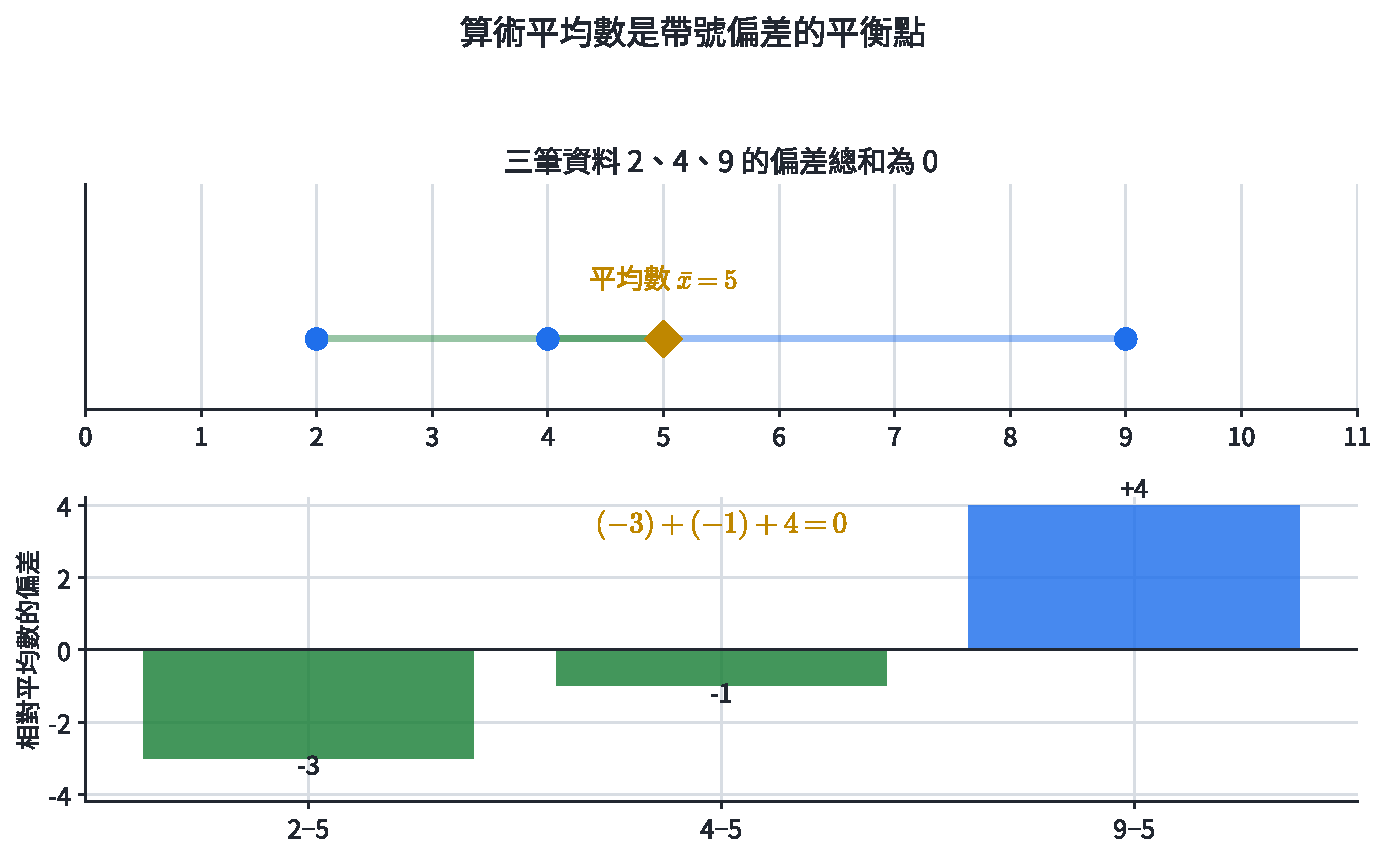
\includegraphics[width=0.92\linewidth,height=\textheight,keepaspectratio,alt={圖 1｜資料 2、4、9 的平均數為 5；三個帶號偏差相加為 0。}]{assets/數2-2-平均數平衡.pdf}
\caption{圖 1｜資料 2、4、9 的平均數為 5；三個帶號偏差相加為 0。}
\end{figure}

若只知道平均數與筆數，仍可還原總和：

\[
\boxed{\sum x_i=n\bar{x}}.
\]

這個關係常用於補遺失資料、合併兩組資料或更新平均數。

\subsection{1.2 加權平均數}\label{ux52a0ux6b0aux5e73ux5747ux6578}

當各數值代表的次數或重要程度不同時，使用權數 \(w_i>0\)：

\[
\boxed{\bar{x}_w=\frac{w_1x_1+w_2x_2+\cdots+w_nx_n}{w_1+w_2+\cdots+w_n}}.
\]

次數分配表中的次數就是權數。若資料值 \(a_1,a_2,\ldots,a_k\) 分別出現 \(f_1,f_2,\ldots,f_k\) 次，則總筆數為 \(N=\sum f_i\)，平均數為

\[
\bar{x}=\frac{\sum f_i a_i}{N}.
\]

\subsection{1.3 幾何平均數與平均成長率}\label{ux5e7eux4f55ux5e73ux5747ux6578ux8207ux5e73ux5747ux6210ux9577ux7387}

算術平均處理相加的量；連續成長則由倍率相乘。\(n\) 個正數 \(x_1,x_2,\ldots,x_n\) 的\textbf{幾何平均數}為

\[
\boxed{G=\sqrt[n]{x_1x_2\cdots x_n}}.
\]

若連續 \(n\) 期的成長率為 \(r_1,r_2,\ldots,r_n\)，每期倍率是 \(1+r_i\)。等效的固定成長率 \(r\) 滿足

\[
(1+r)^n=(1+r_1)(1+r_2)\cdots(1+r_n),
\]

所以

\[
\boxed{r=\sqrt[n]{(1+r_1)(1+r_2)\cdots(1+r_n)}-1}.
\]

這個模型要求每期結束值成為下一期起始值，因此適用於資產、人口、產量等複合增減過程。

\subsection{例 1｜由分組人數計算總平均}\label{ux4f8b-1ux7531ux5206ux7d44ux4ebaux6578ux8a08ux7b97ux7e3dux5e73ux5747}

甲班 24 人的平均成績為 72 分，乙班 16 人的平均成績為 82 分。求兩班合併後的平均成績。

先由「筆數乘平均」還原總分：

\[
S_{\text{甲}}=24\times72,\qquad S_{\text{乙}}=16\times82.
\]

合併後共有 40 人，因此

\[
\bar{x}=\frac{24\times72+16\times82}{40}
=\frac{3040}{40}=\boxed{76\text{ 分}}.
\]

兩班人數不同，直接平均 \(72\) 與 \(82\) 會把兩班誤當成同樣大小；以人數加權才對應全部 40 筆資料。

\subsection{例 2｜三年平均成長率}\label{ux4f8b-2ux4e09ux5e74ux5e73ux5747ux6210ux9577ux7387}

某項產量三年的成長率依序為 \(20\%\)、\(-10\%\)、\(25\%\)。求等效的年平均成長率。

三年的總倍率為

\[
1.20\times0.90\times1.25=1.35.
\]

設等效年平均成長率為 \(r\)，則

\[
(1+r)^3=1.35,\qquad
r=\sqrt[3]{1.35}-1\approx0.1052.
\]

所以等效年平均成長率約為 \(\boxed{10.5\%}\)。驗算：\(1.1052^3\approx1.35\)。

\subsubsection{練習 1A}\label{ux7df4ux7fd2-1a}

\begin{enumerate}
\def\labelenumi{\arabic{enumi}.}
\tightlist
\item
  資料 \(6,7,8,9,10\) 的算術平均數為何？
\item
  某課程的作業、期中考、期末考分數依序為 84、72、90，權重依序為 \(20\%,30\%,50\%\)。求加權成績。
\item
  顧客評價 1、2、3 分分別有 2、5、3 人。求平均評價。
\item
  某數量連續兩年的倍率為 \(1.10\) 與 \(1.21\)。求等效的年平均成長率。
\item
  六筆資料的平均數為 14，其中五筆為 8、11、13、17、19。求第六筆資料。
\end{enumerate}

\subsubsection{練習 1A 解析}\label{ux7df4ux7fd2-1a-ux89e3ux6790}

\begin{enumerate}
\def\labelenumi{\arabic{enumi}.}
\tightlist
\item
  \(\bar{x}=(6+7+8+9+10)/5=\boxed{8}\)。
\item
  \(0.2(84)+0.3(72)+0.5(90)=\boxed{83.4}\) 分。
\item
  總人數為 10，\(\bar{x}=(1\times2+2\times5+3\times3)/10=\boxed{2.1}\) 分。
\item
  \(1+r=\sqrt{1.10\times1.21}=\sqrt{1.331}\approx1.1537\)，故 \(r\approx\boxed{15.4\%}\)。
\item
  六筆總和為 \(6\times14=84\)，已知五筆和為 68，第六筆為 \(\boxed{16}\)。
\end{enumerate}

\section{2. 排序位置：百分位數與盒狀圖}\label{ux6392ux5e8fux4f4dux7f6eux767eux5206ux4f4dux6578ux8207ux76d2ux72c0ux5716}

\subsection{\texorpdfstring{2.1 第 \(m\) 百分位數}{2.1 第 m 百分位數}}\label{ux7b2c-m-ux767eux5206ux4f4dux6578}

第 \(m\) 百分位數記作 \(P_m\)，其中 \(1\le m\le99\)。它代表至少有 \(m\%\) 的資料小於或等於 \(P_m\)，同時至少有 \((100-m)\%\) 的資料大於或等於 \(P_m\)。

本章採用課本約定。先把 \(n\) 筆資料由小到大排成

\[
x_{(1)}\le x_{(2)}\le\cdots\le x_{(n)},
\]

再計算 \(I=nm/100\)。

\begin{itemize}
\tightlist
\item
  若 \(I\) 不是整數，令 \(M=\lceil I\rceil\)，則 \(P_m=x_{(M)}\)。
\item
  若 \(I\) 是整數，則 \(P_m=\dfrac{x_{(I)}+x_{(I+1)}}2\)。
\end{itemize}

同一組資料若採用其他統計軟體的內插規則，數值可能略有差異；書面作答應先確認題目指定的定義。本章計算均依上列規則。

第 1、2、3 四分位數分別為

\[
Q_1=P_{25},\qquad Q_2=P_{50},\qquad Q_3=P_{75}.
\]

\(Q_2\) 就是中位數。四分位距定義為

\[
\boxed{\mathrm{IQR}=Q_3-Q_1},
\]

它描述中間 \(50\%\) 資料占據的範圍，對極端值的反應通常小於全距。

\begin{figure}
\centering
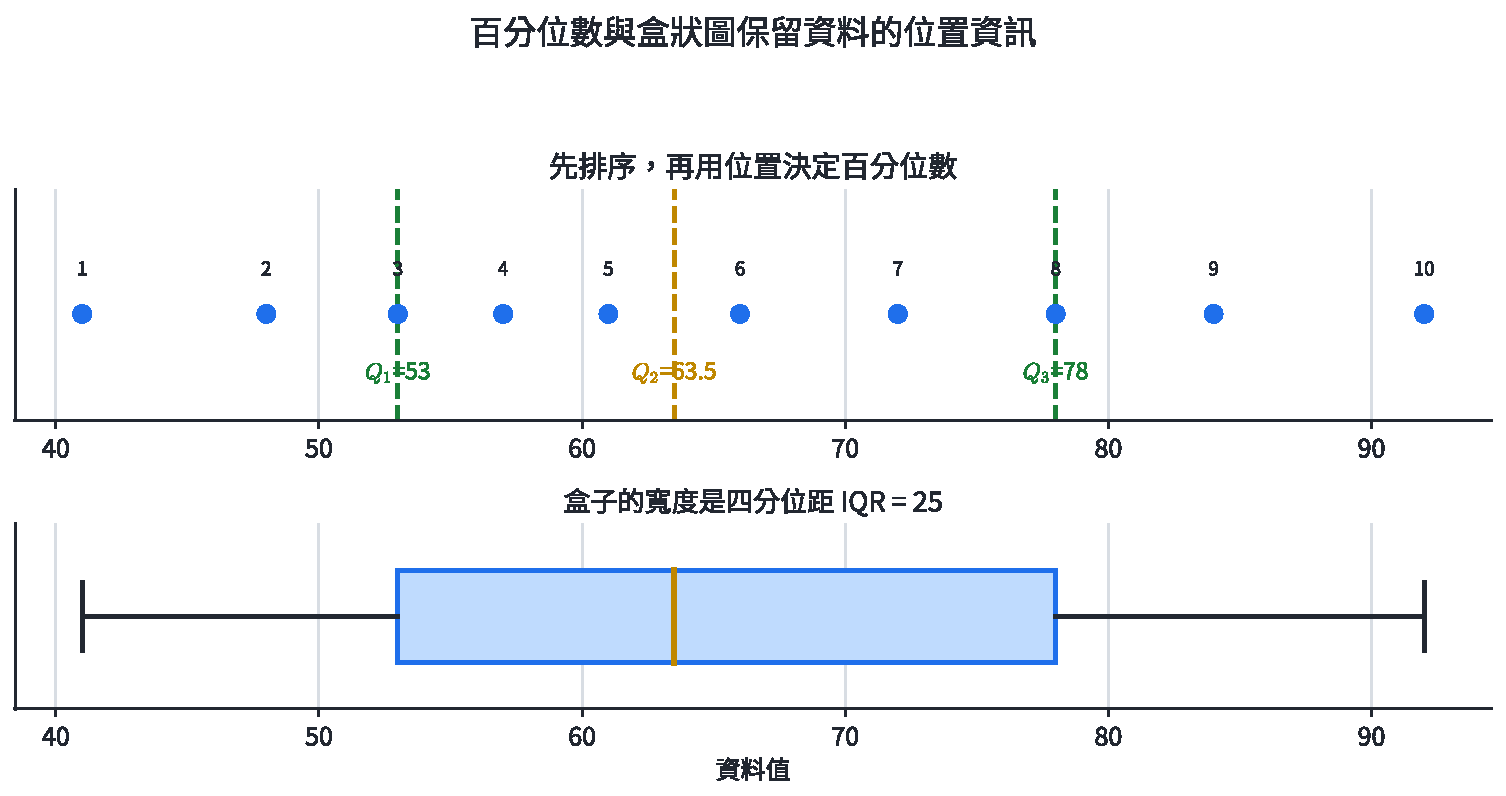
\includegraphics[width=0.94\linewidth,height=\textheight,keepaspectratio,alt={圖 2｜先排序再定位四分位數；盒狀圖依本章百分位數規則繪出五數摘要。}]{assets/數2-2-百分位數與盒狀圖.pdf}
\caption{圖 2｜先排序再定位四分位數；盒狀圖依本章百分位數規則繪出五數摘要。}
\end{figure}

\subsection{2.2 五數摘要與盒狀圖}\label{ux4e94ux6578ux6458ux8981ux8207ux76d2ux72c0ux5716}

盒狀圖用最小值、\(Q_1\)、中位數、\(Q_3\)、最大值五個數描述資料。盒子的左右端是 \(Q_1,Q_3\)，盒內線段是中位數，兩側線段延伸至最小值與最大值。

盒狀圖可以快速比較多組資料的中心、分散與偏斜情形。例如右側鬚明顯較長，表示較大的資料占據較寬範圍；中位數偏向盒子一端，也表示盒內兩半的分散程度不同。

\subsection{例 3｜依排序位置求百分位數}\label{ux4f8b-3ux4f9dux6392ux5e8fux4f4dux7f6eux6c42ux767eux5206ux4f4dux6578}

十筆資料已由小到大排列：

\[
10,13,16,18,22,24,26,28,30,33.
\]

求 \(P_{35}\) 與 \(P_{60}\)。

對 \(P_{35}\)，\(I=10\times0.35=3.5\)。\(3.5\) 不是整數，向上取到第 4 筆，所以 \(\boxed{P_{35}=18}\)。

對 \(P_{60}\)，\(I=10\times0.60=6\)。\(6\) 是整數，取第 6、7 筆平均：

\[
P_{60}=\frac{24+26}{2}=\boxed{25}.
\]

\subsection{例 4｜五數摘要與四分位距}\label{ux4f8b-4ux4e94ux6578ux6458ux8981ux8207ux56dbux5206ux4f4dux8ddd}

資料為 \(2,4,5,7,9,12,14,18\)。求五數摘要與四分位距。

資料已排序且 \(n=8\)。

\[
\begin{aligned}
Q_1&=\frac{x_{(2)}+x_{(3)}}2=\frac{4+5}{2}=4.5,\\
Q_2&=\frac{x_{(4)}+x_{(5)}}2=\frac{7+9}{2}=8,\\
Q_3&=\frac{x_{(6)}+x_{(7)}}2=\frac{12+14}{2}=13.
\end{aligned}
\]

五數摘要為 \(\boxed{(2,4.5,8,13,18)}\)，四分位距為 \(13-4.5=\boxed{8.5}\)。

\subsubsection{練習 2A}\label{ux7df4ux7fd2-2a}

\begin{enumerate}
\def\labelenumi{\arabic{enumi}.}
\tightlist
\item
  九筆已排序資料為 \(3,5,6,8,10,13,15,18,21\)。求 \(P_{40}\)。
\item
  同一組九筆資料的 \(Q_1,Q_2,Q_3\) 為何？
\item
  資料的五數摘要為 \((12,18,24,31,45)\)。求全距與四分位距。
\item
  甲組的中位數為 70、IQR 為 8；乙組的中位數為 66、IQR 為 20。比較中心與中間一半資料的分散。
\item
  某成績的 \(P_{88}=13\) 級分。說明這個數值的排序意義。
\end{enumerate}

\subsubsection{練習 2A 解析}\label{ux7df4ux7fd2-2a-ux89e3ux6790}

\begin{enumerate}
\def\labelenumi{\arabic{enumi}.}
\tightlist
\item
  \(I=9(0.40)=3.6\)，取第 4 筆，故 \(\boxed{P_{40}=8}\)。
\item
  \(P_{25}\) 的位置為 \(2.25\)，取第 3 筆得 \(Q_1=6\)；\(P_{50}\) 的位置為 \(4.5\)，取第 5 筆得 \(Q_2=10\)；\(P_{75}\) 的位置為 \(6.75\)，取第 7 筆得 \(Q_3=15\)。答案為 \(\boxed{(6,10,15)}\)。
\item
  全距 \(=45-12=\boxed{33}\)；IQR \(=31-18=\boxed{13}\)。
\item
  甲組中位數較高，且中間 \(50\%\) 的資料較集中；乙組中心較低，中間 \(50\%\) 占據的範圍較寬。
\item
  至少有 \(88\%\) 的成績小於或等於 13 級分，同時至少有 \(12\%\) 的成績大於或等於 13 級分。
\end{enumerate}

\section{3. 分散程度、線性轉換與標準化}\label{ux5206ux6563ux7a0bux5ea6ux7ddaux6027ux8f49ux63dbux8207ux6a19ux6e96ux5316}

\subsection{3.1 變異數與標準差}\label{ux8b8aux7570ux6578ux8207ux6a19ux6e96ux5dee}

偏差的總和恆為 0，所以直接平均偏差無法描述分散程度。把偏差平方後再平均，得到\textbf{變異數}：

\[
\boxed{s_x^2=\frac1n\sum_{i=1}^{n}(x_i-\bar{x})^2}.
\]

本章資料視為完整的一組，分母使用 \(n\)。變異數的單位是原單位的平方；開平方後得到與原資料同單位的\textbf{標準差}：

\[
\boxed{s_x=\sqrt{\frac1n\sum_{i=1}^{n}(x_i-\bar{x})^2}}.
\]

展開平方可得到常用計算式：

\[
\begin{aligned}
s_x^2
&=\frac1n\sum(x_i^2-2x_i\bar{x}+\bar{x}^2)\\
&=\frac1n\sum x_i^2-2\bar{x}\left(\frac1n\sum x_i\right)+\bar{x}^2\\
&=\boxed{\frac1n\sum x_i^2-\bar{x}^2}.
\end{aligned}
\]

\begin{figure}
\centering
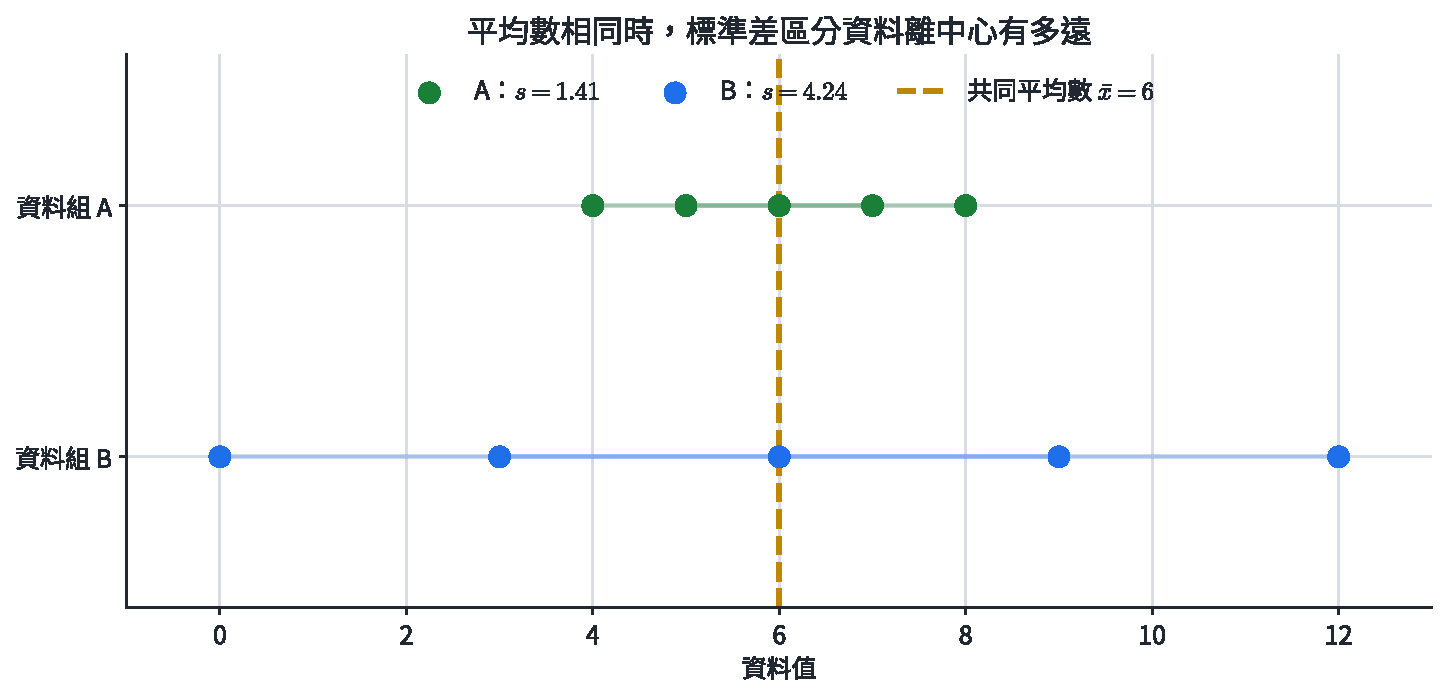
\includegraphics[width=0.91\linewidth,height=\textheight,keepaspectratio,alt={圖 3｜兩組資料都有平均數 6；資料 B 到中心的距離較大，因此標準差較大。}]{assets/數2-2-同平均不同分散.pdf}
\caption{圖 3｜兩組資料都有平均數 6；資料 B 到中心的距離較大，因此標準差較大。}
\end{figure}

\subsection{3.2 資料的伸縮與平移}\label{ux8cc7ux6599ux7684ux4f38ux7e2eux8207ux5e73ux79fb}

若每筆資料都經過相同轉換 \(y_i=ax_i+b\)，則

\[
\boxed{\bar{y}=a\bar{x}+b},
\qquad
\boxed{s_y=|a|s_x}.
\]

第一式由平均數的線性性質直接得到。第二式來自

\[
y_i-\bar{y}=a(x_i-\bar{x}),
\]

每個偏差都乘上 \(a\)，平方平均後乘上 \(a^2\)，再開平方得到 \(|a|\)。加上常數 \(b\) 會把所有資料一起平移，彼此距離不變，所以標準差不受 \(b\) 影響。

\begin{figure}
\centering
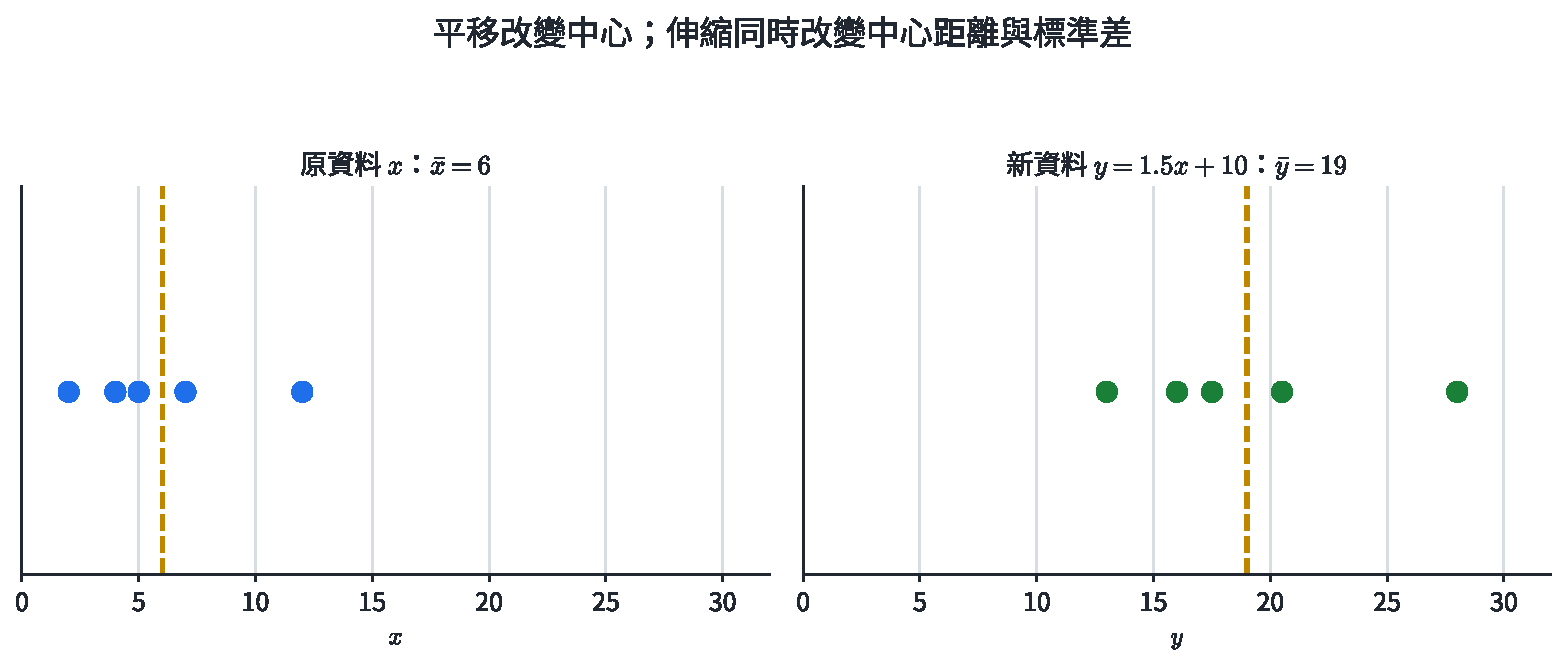
\includegraphics[width=0.94\linewidth,height=\textheight,keepaspectratio,alt={圖 4｜線性轉換的平移改變中心，伸縮改變資料間距。}]{assets/數2-2-資料伸縮平移.pdf}
\caption{圖 4｜線性轉換的平移改變中心，伸縮改變資料間距。}
\end{figure}

\subsection{3.3 標準化數據}\label{ux6a19ux6e96ux5316ux6578ux64da}

當 \(s_x>0\) 時，第 \(i\) 筆資料的\textbf{標準化數據}或 \textbf{z 分數}為

\[
\boxed{z_i=\frac{x_i-\bar{x}}{s_x}}.
\]

\(z_i\) 的正負表示資料在平均數哪一側，\(|z_i|\) 表示距離平均數幾個標準差。全部 z 分數的平均為 0、標準差為 1：

\[
\bar z=\frac1n\sum\frac{x_i-\bar x}{s_x}=0,
\]

\[
s_z^2=\frac1n\sum\left(\frac{x_i-\bar x}{s_x}\right)^2=1.
\]

\begin{figure}
\centering
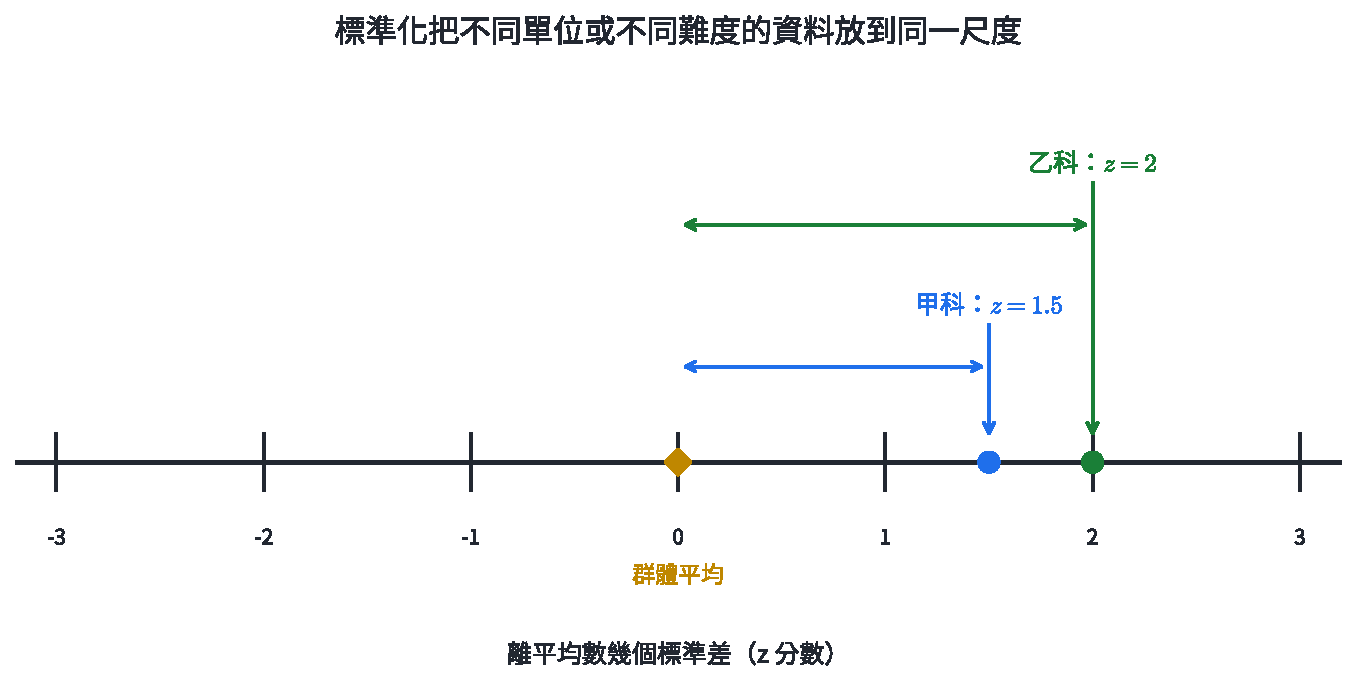
\includegraphics[width=0.91\linewidth,height=\textheight,keepaspectratio,alt={圖 5｜z 分數把不同考試的原始分數轉成離各自平均數的標準差數。}]{assets/數2-2-標準化比較.pdf}
\caption{圖 5｜z 分數把不同考試的原始分數轉成離各自平均數的標準差數。}
\end{figure}

\subsection{例 5｜由偏差平方計算標準差}\label{ux4f8b-5ux7531ux504fux5deeux5e73ux65b9ux8a08ux7b97ux6a19ux6e96ux5dee}

資料為 \(2,4,4,6,9\)。平均數為 \(5\)，偏差平方和為

\[
(-3)^2+(-1)^2+(-1)^2+1^2+4^2=28.
\]

因此

\[
s_x^2=\frac{28}{5}=5.6,\qquad
s_x=\sqrt{5.6}\approx\boxed{2.37}.
\]

平均數與原資料同單位，變異數使用平方單位，標準差回到原單位。

\subsection{例 6｜攝氏與華氏資料的統計量}\label{ux4f8b-6ux651dux6c0fux8207ux83efux6c0fux8cc7ux6599ux7684ux7d71ux8a08ux91cf}

一組攝氏溫度的平均為 \(18^\circ\mathrm C\)、標準差為 \(4^\circ\mathrm C\)。華氏溫度為 \(F=1.8C+32\)。求華氏資料的平均與標準差。

\[
\bar F=1.8(18)+32=\boxed{64.4^\circ\mathrm F},
\]

\[
s_F=|1.8|\times4=\boxed{7.2^\circ\mathrm F}.
\]

轉換中的 \(32\) 只改變中心；倍率 \(1.8\) 同時放大中心差與資料間距。

\subsection{例 7｜比較不同考試中的相對表現}\label{ux4f8b-7ux6bd4ux8f03ux4e0dux540cux8003ux8a66ux4e2dux7684ux76f8ux5c0dux8868ux73fe}

某生甲科 72 分，班平均 60 分、標準差 8 分；乙科 82 分，班平均 70 分、標準差 6 分。

\[
z_{\text{甲}}=\frac{72-60}{8}=1.5,
\qquad
z_{\text{乙}}=\frac{82-70}{6}=2.
\]

乙科成績高於該科平均 2 個標準差，甲科高於平均 1.5 個標準差，因此乙科的相對位置較高。

\subsubsection{練習 3A}\label{ux7df4ux7fd2-3a}

\begin{enumerate}
\def\labelenumi{\arabic{enumi}.}
\tightlist
\item
  資料 \(1,3,5,7\) 的平均數、變異數與標準差為何？
\item
  一組資料平均為 50、標準差為 6。每筆都加 12 後，新平均與新標準差為何？
\item
  承上題，若再把新資料全部乘以 \(-2\)，平均與標準差為何？
\item
  某測量值為 84，該組平均為 72、標準差為 8。求 z 分數並解釋。
\item
  一組標準差為 0 的資料具有什麼共同特徵？
\item
  兩組資料 A、B 的平均都是 20，標準差分別為 3 與 9。某筆資料在 A 中是 26，在 B 中是 32；比較兩筆資料的相對位置。
\end{enumerate}

\subsubsection{練習 3A 解析}\label{ux7df4ux7fd2-3a-ux89e3ux6790}

\begin{enumerate}
\def\labelenumi{\arabic{enumi}.}
\tightlist
\item
  \(\bar{x}=4\)；偏差平方和 \(=9+1+1+9=20\)，所以 \(s^2=5\)、\(s=\boxed{\sqrt5}\)。
\item
  平移 12：新平均 \(\boxed{62}\)，標準差仍為 \(\boxed{6}\)。
\item
  乘以 \(-2\)：平均為 \(\boxed{-124}\)，標準差為 \(|-2|\times6=\boxed{12}\)。
\item
  \(z=(84-72)/8=\boxed{1.5}\)，表示該值高於平均 1.5 個標準差。
\item
  每筆資料都等於平均數，因此全部資料相同。
\item
  \(z_A=(26-20)/3=2\)，\(z_B=(32-20)/9=4/3\)；A 中的資料相對位置較高。
\end{enumerate}

\section{4. 二維數據：散布圖與相關係數}\label{ux4e8cux7dadux6578ux64daux6563ux5e03ux5716ux8207ux76f8ux95dcux4fc2ux6578}

\subsection{4.1 成對資料與散布圖}\label{ux6210ux5c0dux8cc7ux6599ux8207ux6563ux5e03ux5716}

二維數據由成對觀測值

\[
(x_1,y_1),(x_2,y_2),\ldots,(x_n,y_n)
\]

組成。每一對必須來自同一個觀測單位，例如同一位學生的讀書時間與成績、同一天的溫度與用電量。把各對資料畫成平面上的點，就得到\textbf{散布圖}。

散布圖先判讀方向、形狀、緊密程度與特殊點。方向記錄 \(x\) 增加時 \(y\) 大致增加或減少；形狀區分直線、曲線或分群；緊密程度比較點群離主要形狀的距離；特殊點包含離群值與對模型有高度影響的點。

\begin{figure}
\centering
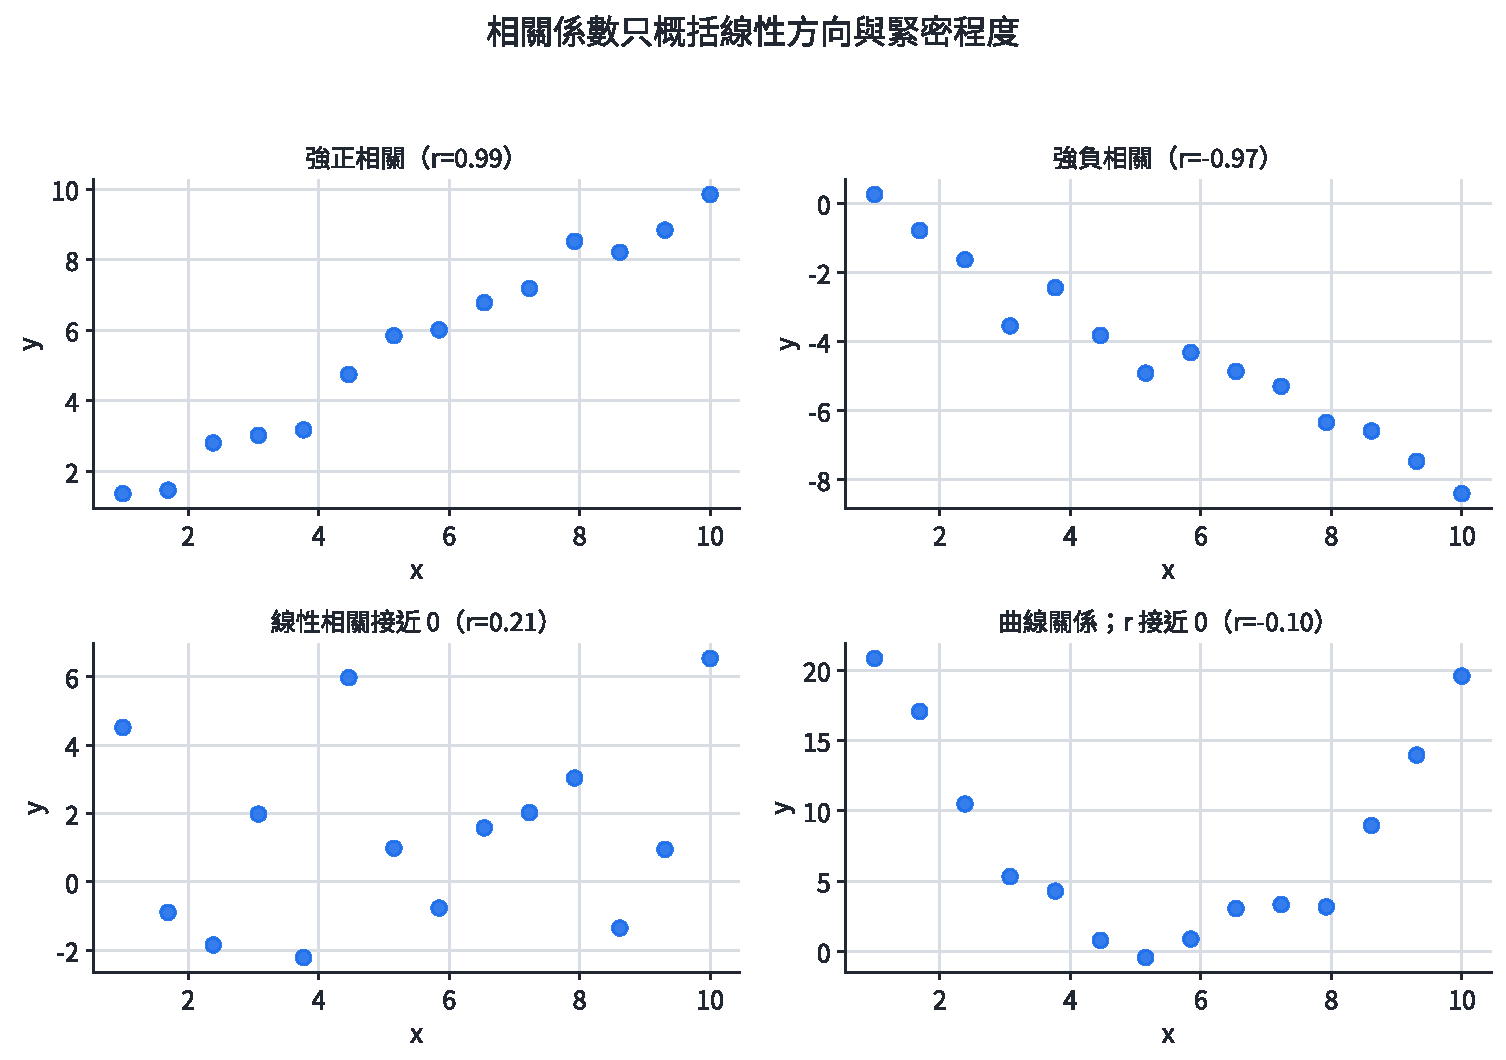
\includegraphics[width=0.94\linewidth,height=\textheight,keepaspectratio,alt={圖 6｜四種散布型態；相關係數概括線性訊號，散布圖保留資料形狀。}]{assets/數2-2-散布圖型態.pdf}
\caption{圖 6｜四種散布型態；相關係數概括線性訊號，散布圖保留資料形狀。}
\end{figure}

\subsection{4.2 相關係數}\label{ux76f8ux95dcux4fc2ux6578}

設 \(x,y\) 的平均數與標準差分別為 \(\bar x,s_x\) 與 \(\bar y,s_y\)，且 \(s_x,s_y>0\)。皮爾森相關係數定義為

\[
\boxed{r=\frac1n\sum_{i=1}^{n}\frac{x_i-\bar x}{s_x}\frac{y_i-\bar y}{s_y}}
=\boxed{\frac{\frac1n\sum(x_i-\bar x)(y_i-\bar y)}{s_xs_y}}.
\]

當一筆資料的 \(x,y\) 同時高於各自平均，或同時低於各自平均，兩個 z 分數乘積為正；一高一低時乘積為負。因此 \(r\) 的正負表示線性方向。

由柯西不等式

\[
\left(\sum z_{x_i}z_{y_i}\right)^2
\le\left(\sum z_{x_i}^2\right)\left(\sum z_{y_i}^2\right)=n^2,
\]

可得 \(\boxed{-1\le r\le1}\)。\(r=1\) 表示所有點落在正斜率直線上，\(r=-1\) 表示落在負斜率直線上。\(|r|\) 越接近 1，線性排列越緊密；\(r\) 接近 0 只表示線性訊號弱，散布圖仍可能呈現曲線或分群。

若 \(X'=aX+b\)、\(Y'=cY+d\)，其中 \(a,c\ne0\)，則

\[
r_{X',Y'}=\operatorname{sgn}(ac)r_{X,Y}.
\]

平移不改變相關係數；正倍率保留方向，負倍率翻轉方向。

\subsection{4.3 離群值與解釋範圍}\label{ux96e2ux7fa4ux503cux8207ux89e3ux91cbux7bc4ux570d}

相關係數會受少數遠離點群的資料影響。報告 \(r\) 前應先看散布圖，確認點的配對、形狀、範圍與特殊點。

\begin{figure}
\centering
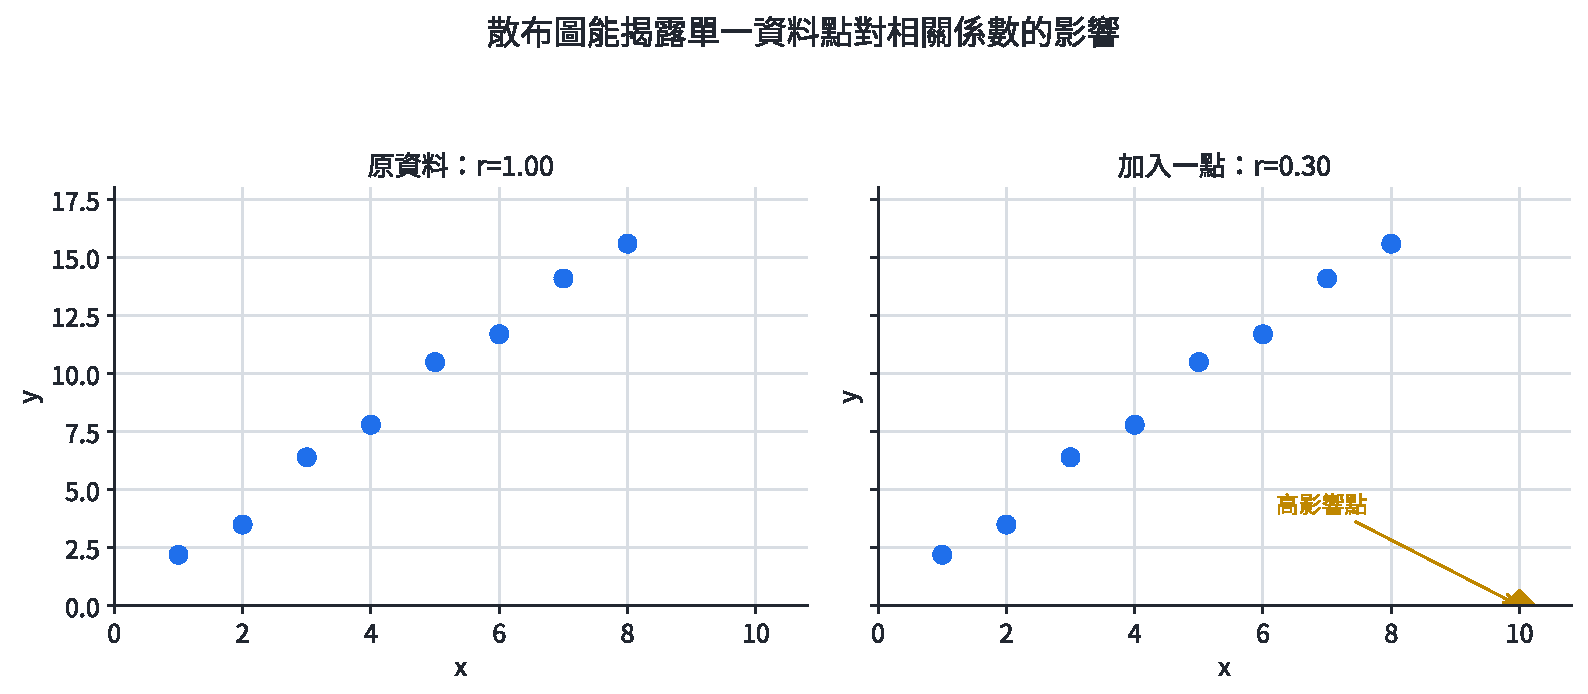
\includegraphics[width=0.92\linewidth,height=\textheight,keepaspectratio,alt={圖 7｜加入一個高影響點後，相關係數由接近 1 明顯下降。}]{assets/數2-2-離群值影響.pdf}
\caption{圖 7｜加入一個高影響點後，相關係數由接近 1 明顯下降。}
\end{figure}

相關反映共同變動，因果關係還需要時間順序、控制變因、機制與實驗或其他證據。例如冰品銷量與用電量可能同時隨氣溫上升，兩者的相關不等於其中一者造成另一者。

\subsection{例 8｜完全正線性相關}\label{ux4f8b-8ux5b8cux5168ux6b63ux7ddaux6027ux76f8ux95dc}

資料為 \((1,2),(2,4),(3,6),(4,8)\)。每一點都滿足 \(y=2x\)，標準化後有 \(z_{y_i}=z_{x_i}\)，所以

\[
r=\frac1n\sum z_{x_i}^2=\boxed{1}.
\]

直線斜率為 2，而相關係數為 1；相關係數沒有單位，也不等於原圖斜率。

\subsection{例 9｜由偏差表計算相關係數}\label{ux4f8b-9ux7531ux504fux5deeux8868ux8a08ux7b97ux76f8ux95dcux4fc2ux6578}

四對資料為 \((1,4),(2,1),(3,3),(4,2)\)。\(x,y\) 的平均數都為 \(2.5\)，標準差都為 \(\sqrt{1.25}\)。偏差乘積和為

\[
(-1.5)(1.5)+(-0.5)(-1.5)+(0.5)(0.5)+(1.5)(-0.5)=-2.
\]

因此

\[
r=\frac{(-2)/4}{\sqrt{1.25}\sqrt{1.25}}=\frac{-0.5}{1.25}=\boxed{-0.4}.
\]

資料呈負線性方向；完整判讀仍需配合散布圖。

\subsection{例 10｜單位轉換對相關係數的影響}\label{ux4f8b-10ux55aeux4f4dux8f49ux63dbux5c0dux76f8ux95dcux4fc2ux6578ux7684ux5f71ux97ff}

身高 \(H\) 以公分表示，體重為 \(W\)，已知 \(r_{H,W}=0.72\)。若改用英吋 \(H'=H/2.54\)，並定義指標 \(K=100-W\)，求 \(r_{H',K}\)。

\(H'\) 對 \(H\) 是正倍率轉換，保留方向；\(K\) 對 \(W\) 是負倍率加平移，翻轉方向。因此 \(\boxed{r_{H',K}=-0.72}\)。

\subsubsection{練習 4A}\label{ux7df4ux7fd2-4a}

\begin{enumerate}
\def\labelenumi{\arabic{enumi}.}
\tightlist
\item
  散布點由左下向右上形成狹長帶狀，相關係數的符號與大致大小如何？
\item
  若所有資料滿足 \(y=7-3x\) 且 \(x\) 不全相同，求 \(r\)。
\item
  已知 \(r_{X,Y}=-0.65\)。求 \(r_{2X+5,,4Y-1}\) 與 \(r_{-X,,4Y-1}\)。
\item
  某資料的 \(r=0.03\)，散布圖呈清楚的 U 形。應如何描述兩變量關係？
\item
  一份資料把不同學生的身高與體重分別排序後再任意配對。這個散布圖能否代表原來的身高---體重關係？說明理由。
\item
  廣告費與銷售額高度正相關。列出一項仍需檢查、才能支持「提高廣告費造成銷售增加」的證據。
\end{enumerate}

\subsubsection{練習 4A 解析}\label{ux7df4ux7fd2-4a-ux89e3ux6790}

\begin{enumerate}
\def\labelenumi{\arabic{enumi}.}
\tightlist
\item
  符號為正，且 \(|r|\) 接近 1；實際數值仍須由資料計算。
\item
  全部點落在負斜率直線上，所以 \(\boxed{r=-1}\)。
\item
  兩個正倍率保留方向，第一式為 \(\boxed{-0.65}\)；第一個倍率為負，第二式為 \(\boxed{0.65}\)。
\item
  兩變量的線性相關接近 0，但存在明顯非線性關係；U 形結構由散布圖提供。
\item
  無法。二維資料的每一對觀測必須來自同一位學生，任意重配會改變共同變動資訊。
\item
  可檢查隨機或合理控制下的實驗結果、廣告投入先於銷售改變的時間資料，並控制季節、價格與促銷等共同因素。任列一項且說明作用即可。
\end{enumerate}

\section{5. 最小平方直線與殘差}\label{ux6700ux5c0fux5e73ux65b9ux76f4ux7ddaux8207ux6b98ux5dee}

\subsection{5.1 預測值與殘差}\label{ux9810ux6e2cux503cux8207ux6b98ux5dee}

用直線 \(\hat y=a+bx\) 預測 \(y\) 時，第 \(i\) 筆的預測值為 \(\hat y_i=a+bx_i\)，\textbf{殘差}為

\[
\boxed{e_i=y_i-\hat y_i}.
\]

殘差是散布點到直線的鉛直帶號距離。最小平方直線選擇 \(a,b\)，使殘差平方和

\[
\mathrm{SSE}=\sum_{i=1}^{n}(y_i-a-bx_i)^2
\]

達到最小。

\begin{figure}
\centering
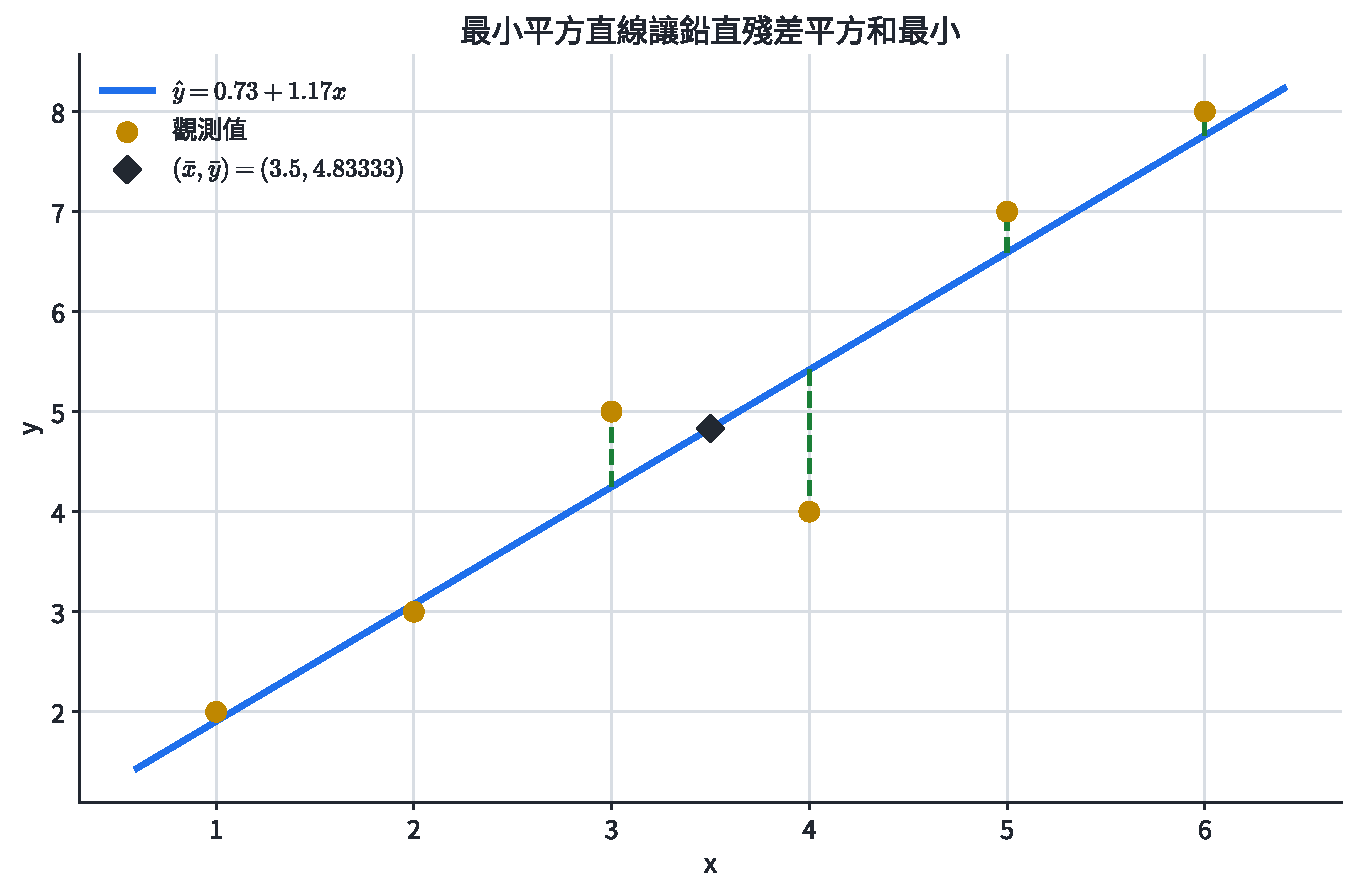
\includegraphics[width=0.91\linewidth,height=\textheight,keepaspectratio,alt={圖 8｜每一條綠色虛線是一個殘差；最小平方直線通過 (\textbackslash bar x,\textbackslash bar y)。}]{assets/數2-2-最小平方法.pdf}
\caption{圖 8｜每一條綠色虛線是一個殘差；最小平方直線通過 \((\bar x,\bar y)\)。}
\end{figure}

\subsection{5.2 迴歸係數的推導}\label{ux8ff4ux6b78ux4fc2ux6578ux7684ux63a8ux5c0e}

固定 \(b\) 時，將 \(y_i-a-bx_i=(y_i-bx_i)-a\) 視為一組數據到常數 \(a\) 的距離。平方和在 \(a\) 等於這組數據的平均時最小，因此

\[
a=\bar y-b\bar x.
\]

代回後，令 \(u_i=x_i-\bar x\)、\(v_i=y_i-\bar y\)，則

\[
\begin{aligned}
\mathrm{SSE}
&=\sum(v_i-bu_i)^2\\
&=\sum v_i^2-2b\sum u_iv_i+b^2\sum u_i^2.
\end{aligned}
\]

這是以 \(b\) 為變數、開口向上的二次式。配方後最小值出現在

\[
\boxed{b=\frac{\sum(x_i-\bar x)(y_i-\bar y)}{\sum(x_i-\bar x)^2}}
=\boxed{r\frac{s_y}{s_x}}.
\]

截距為 \(\boxed{a=\bar y-b\bar x}\)，所以最小平方直線必通過 \((\bar x,\bar y)\)。斜率 \(b\) 帶有 \(y\) 單位除以 \(x\) 單位，表示 \(x\) 每增加 1 單位時，模型預測的 \(y\) 平均改變量。

在標準化坐標中，迴歸式簡化為

\[
\boxed{\hat z_y=r z_x}.
\]

\subsection{5.3 使用範圍與殘差判讀}\label{ux4f7fux7528ux7bc4ux570dux8207ux6b98ux5deeux5224ux8b80}

線性預測適用於散布圖在觀測範圍內大致呈直線的資料。若殘差圖仍呈彎曲、漏斗狀或分群，代表直線尚未捕捉主要結構。遠離觀測範圍的外插會依賴未被資料驗證的趨勢，預測不確定性通常更高。

迴歸線預測的是群體中的典型 \(y\)，個別觀測仍可能因未納入變量與隨機差異偏離直線。殘差的單位與 \(y\) 相同，正殘差表示實際值高於預測值。

\subsection{例 11｜建立最小平方直線}\label{ux4f8b-11ux5efaux7acbux6700ux5c0fux5e73ux65b9ux76f4ux7dda}

六對資料為 \((1,2),(2,3),(3,5),(4,4),(5,7),(6,8)\)。計算得

\[
\bar x=3.5,\qquad \bar y=\frac{29}{6},
\]

\[
\sum(x_i-\bar x)^2=\frac{35}{2},
\qquad
\sum(x_i-\bar x)(y_i-\bar y)=\frac{41}{2}.
\]

因此

\[
b=\frac{41}{35},
\qquad
a=\frac{29}{6}-\frac{41}{35}\cdot\frac72=\frac{11}{15}.
\]

最小平方直線為

\[
\boxed{\hat y=\frac{11}{15}+\frac{41}{35}x}
\approx0.733+1.171x.
\]

用 \(x=7\) 預測得 \(\hat y\approx8.93\)。這只比原資料最大 \(x=6\) 多 1，屬鄰近外插，仍應標示預測性質。

\subsection{例 12｜由摘要統計量寫出迴歸式}\label{ux4f8b-12ux7531ux6458ux8981ux7d71ux8a08ux91cfux5bebux51faux8ff4ux6b78ux5f0f}

某資料有 \(\bar x=40,s_x=5,\bar y=70,s_y=8,r=0.75\)。求以 \(x\) 預測 \(y\) 的最小平方直線，並預測 \(x=46\) 時的 \(y\)。

\[
b=r\frac{s_y}{s_x}=0.75\cdot\frac85=1.2.
\]

用通過平均點的形式：

\[
\hat y-70=1.2(x-40),
\]

故 \(\boxed{\hat y=22+1.2x}\)。代入 \(x=46\) 得 \(\hat y=\boxed{77.2}\)。

\subsection{例 13｜用殘差平方和比較直線}\label{ux4f8b-13ux7528ux6b98ux5deeux5e73ux65b9ux548cux6bd4ux8f03ux76f4ux7dda}

資料為 \((1,2),(2,3),(3,5)\)。資料平均為 \(\bar x=2,\bar y=10/3\)，最小平方直線為

\[
\hat y=\frac13+\frac32x.
\]

三個殘差依序為 \(1/6,-1/3,1/6\)，所以

\[
\mathrm{SSE}_{\mathrm{LS}}=\frac1{36}+\frac19+\frac1{36}=\frac16.
\]

對候選直線 \(y=x+1\)，三個殘差為 \(0,0,1\)，所以 \(\mathrm{SSE}_{x+1}=1\)。\(1/6<1\)，數值驗證最小平方直線的平方誤差較小。

\subsubsection{練習 5A}\label{ux7df4ux7fd2-5a}

\begin{enumerate}
\def\labelenumi{\arabic{enumi}.}
\tightlist
\item
  已知 \(\bar x=10,s_x=2,\bar y=30,s_y=6,r=0.5\)。求以 \(x\) 預測 \(y\) 的迴歸式。
\item
  承上題，當 \(x=14\) 時的預測值為何？
\item
  某點的實際值為 42，模型預測值為 39.5。求殘差並說明正負。
\item
  最小平方直線為 \(\hat y=5-0.8x\)。把 \(x\) 增加 3 單位時，預測 \(y\) 改變多少？
\item
  已知 \(z_x=1.5,r=-0.6\)。求預測的 \(z_y\)。
\item
  一份資料的 \(x\) 範圍為 20 至 40，模型被拿來預測 \(x=100\)。指出這項預測需要揭露的限制。
\end{enumerate}

\subsubsection{練習 5A 解析}\label{ux7df4ux7fd2-5a-ux89e3ux6790}

\begin{enumerate}
\def\labelenumi{\arabic{enumi}.}
\tightlist
\item
  \(b=0.5(6/2)=1.5\)，所以 \(\hat y-30=1.5(x-10)\)，即 \(\boxed{\hat y=15+1.5x}\)。
\item
  \(\hat y=15+1.5(14)=\boxed{36}\)。
\item
  \(e=42-39.5=\boxed{2.5}\)；正值表示實際值高於模型預測。
\item
  \(\Delta\hat y=-0.8(3)=\boxed{-2.4}\)，預測值下降 2.4 單位。
\item
  \(\hat z_y=rz_x=(-0.6)(1.5)=\boxed{-0.9}\)。
\item
  \(x=100\) 遠超出觀測範圍，屬遠距外插；資料沒有驗證直線趨勢在該處仍成立，預測不確定性較高。
\end{enumerate}

\section{6. 代表題與跨節整合題}\label{ux4ee3ux8868ux984cux8207ux8de8ux7bc0ux6574ux5408ux984c}

\subsection{基礎與核心題}\label{ux57faux790eux8207ux6838ux5fc3ux984c}

\begin{enumerate}
\def\labelenumi{\arabic{enumi}.}
\tightlist
\item
  八筆資料的平均數為 15。加入一筆 24 後，新平均數為何？
\item
  某投資兩年的報酬率依序為 \(44\%\) 與 \(-19\%\)。求等效年平均報酬率。
\item
  十二筆由小到大排列的資料中，第 3、4 筆為 18、21，第 6、7 筆為 29、31，第 9、10 筆為 42、50。求 \(Q_1,Q_2,Q_3\)。
\item
  甲組資料的五數摘要為 \((10,18,25,31,48)\)，乙組為 \((8,21,24,28,40)\)。比較兩組中位數、IQR 與全距。
\item
  資料 \(3,3,7,7\) 的平均數與標準差為何？
\item
  一組資料平均為 12、標準差為 5。新資料定義為 \(Y=20-3X\)。求 \(Y\) 的平均與標準差。
\item
  某生分數 76，群體平均 64、標準差 10。求 z 分數。
\item
  已知 \(r_{X,Y}=0.84\)。求 \(r_{5-2X,,3Y+7}\)。
\end{enumerate}

\subsection{推理與資料題}\label{ux63a8ux7406ux8207ux8cc7ux6599ux984c}

\begin{enumerate}
\def\labelenumi{\arabic{enumi}.}
\setcounter{enumi}{8}
\tightlist
\item
  某散布圖的點完整落在圓周上。說明為何僅報告 \(r\) 無法完整描述 \(X,Y\) 關係。
\item
  五對資料的標準化數據乘積依序為 \(0.8,1.1,-0.2,0.4,0.9\)。求相關係數。
\item
  已知 \(\bar x=50,s_x=10,\bar y=120,s_y=15,r=-0.8\)。求以 \(x\) 預測 \(y\) 的最小平方直線。
\item
  模型為 \(\hat y=18+2.4x\)。觀測 \((x,y)=(5,33)\) 的殘差為何？若另一點殘差為 \(-4\)，它在迴歸線哪一側？
\end{enumerate}

\subsection{跨節整合題}\label{ux8de8ux7bc0ux6574ux5408ux984c}

\begin{enumerate}
\def\labelenumi{\arabic{enumi}.}
\setcounter{enumi}{12}
\tightlist
\item
  某班原始成績平均 68、標準差 8。教師採用新分數 \(Y=1.25X+5\)。學生甲原始成績 84。求新分數的平均、標準差及甲的原始與新制 z 分數，並說明相對位置是否改變。
\item
  八筆每日氣溫與用電量資料的摘要為 \(\bar x=28^\circ\mathrm C,s_x=2^\circ\mathrm C,\bar y=420\text{ kWh},s_y=30\text{ kWh},r=0.7\)。求迴歸式，預測 \(30^\circ\mathrm C\) 的用電量，並說明把此式用於 \(45^\circ\mathrm C\) 的主要限制。
\item
  某組十筆資料加入一筆遠離點群的資料後，\(x\) 平均由 20 變為 23。求新加入資料的 \(x\) 值。加入前 \(r=0.91\)，加入後 \(r=0.28\)；依這些資訊提出合理的資料檢查流程。
\item
  兩地跑步成績以秒記錄。甲地平均 780 秒、標準差 60 秒；乙地平均 720 秒、標準差 40 秒。選手 A 在甲地跑 690 秒，選手 B 在乙地跑 660 秒。以 z 分數比較相對表現；再說明「時間越短越好」如何影響結論的語意。
\end{enumerate}

\section{7. 完整詳解}\label{ux5b8cux6574ux8a73ux89e3}

\begin{enumerate}
\def\labelenumi{\arabic{enumi}.}
\item
  原八筆總和為 \(8\times15=120\)。加入 24 後總和 144、筆數 9，所以新平均為 \(\boxed{16}\)。
\item
  兩年總倍率為 \(1.44\times0.81=1.1664\)。設等效年平均報酬率為 \(r\)，則 \(1+r=\sqrt{1.1664}=1.08\)，因此 \(\boxed{r=8\%}\)。
\item
  \(n=12\)。\(Q_1\) 的位置為 3，取第 3、4 筆平均，得 \(Q_1=19.5\)；\(Q_2\) 的位置為 6，得 \(Q_2=30\)；\(Q_3\) 的位置為 9，得 \(Q_3=46\)。故 \(\boxed{(Q_1,Q_2,Q_3)=(19.5,30,46)}\)。
\item
  甲、乙中位數分別為 25、24，甲較高 1。IQR 分別為 \(31-18=13\)、\(28-21=7\)，乙組中間一半較集中。全距分別為 \(48-10=38\)、\(40-8=32\)，乙組整體範圍也較小。
\item
  平均數為 \(5\)。偏差為 \(-2,-2,2,2\)，所以 \(s=\sqrt{(4+4+4+4)/4}=\boxed{2}\)。
\item
  \(\bar Y=20-3(12)=\boxed{-16}\)；\(s_Y=|-3|(5)=\boxed{15}\)。負倍率翻轉資料次序，但標準差取距離大小。
\item
  \(z=(76-64)/10=\boxed{1.2}\)，表示成績高於群體平均 1.2 個標準差。
\item
  \(5-2X\) 的倍率為負，\(3Y+7\) 的倍率為正，因此相關方向翻轉，大小不變：\(\boxed{-0.84}\)。
\item
  圓周呈明顯的非線性封閉關係。同一個 \(x\) 可能對應上下兩個 \(y\)，整體正、負偏差乘積可能互相抵銷，使 \(r\) 接近 0。應同時呈現散布圖並描述曲線結構。
\item
  \(r=(0.8+1.1-0.2+0.4+0.9)/5=3.0/5=\boxed{0.6}\)。
\item
  斜率 \(b=-0.8(15/10)=-1.2\)。迴歸線通過 \((50,120)\)：

  \[
  \hat y-120=-1.2(x-50),
  \]

  所以 \(\boxed{\hat y=180-1.2x}\)。
\item
  \(x=5\) 時，\(\hat y=18+2.4(5)=30\)，殘差 \(e=33-30=\boxed{3}\)。殘差 \(-4\) 表示實際值比預測值低 4，點位於迴歸線下方。
\item
  新平均與標準差為

  \[
  \bar Y=1.25(68)+5=90,
  \qquad
  s_Y=1.25(8)=10.
  \]

  甲的新分數為 \(1.25(84)+5=110\)。兩種制度的 z 分數皆為 2：

  \[
  z_X=\frac{84-68}{8}=2,
  \qquad
  z_Y=\frac{110-90}{10}=2.
  \]

  正倍率線性轉換保留標準化位置，因此相對位置不變。
\item
  斜率 \(b=0.7(30/2)=10.5\ \text{kWh}/^\circ\text C\)。迴歸式為

  \[
  \hat y-420=10.5(x-28),
  \]

  即 \(\boxed{\hat y=126+10.5x}\)。\(x=30\) 時，\(\hat y=441\text{ kWh}\)。\(45^\circ\mathrm C\) 遠離觀測範圍，線性趨勢是否持續缺乏資料支持；設備容量與用電行為也可能在極端高溫改變。
\item
  原十筆總和為 \(10(20)=200\)。加入後共 11 筆、總和 \(11(23)=253\)，所以新資料的 \(x\) 值為 \(\boxed{53}\)。檢查流程可依序為：回查原始紀錄與單位、確認它是否屬於同一觀測族群、比較含與不含該點的散布圖與相關係數、說明保留或排除的資料理由。\(r\) 的大幅下降顯示這一點具有高度影響。
\item
  秒數的 z 分數為

  \[
  z_A=\frac{690-780}{60}=-1.5,
  \qquad
  z_B=\frac{660-720}{40}=-1.5.
  \]

  兩人都比所在地平均快 1.5 個標準差，相對表現相同。此處較小的時間代表較佳表現，所以負 z 分數在語意上是高於平均的運動表現；z 的正負只描述數值方向，優劣取決於變量意義。
\end{enumerate}

\section{8. 核心整理}\label{ux6838ux5fc3ux6574ux7406}

\begin{itemize}
\tightlist
\item
  中心：\(\bar x=\dfrac1n\sum x_i\)；不同權重使用 \(\bar x_w=\dfrac{\sum w_ix_i}{\sum w_i}\)；連續倍率使用幾何平均。
\item
  排序：依課本規則先算 \(I=nm/100\)；非整數取第 \(\lceil I\rceil\) 筆，整數取第 \(I\)、\(I+1\) 筆平均。
\item
  分散：\(s_x^2=\dfrac1n\sum(x_i-\bar x)^2=\dfrac1n\sum x_i^2-\bar x^2\)，\(s_x=\sqrt{s_x^2}\)。
\item
  轉換：若 \(Y=aX+b\)，則 \(\bar Y=a\bar X+b\)、\(s_Y=|a|s_X\)。
\item
  標準化：\(z=(x-\bar x)/s_x\)，整組 z 分數平均為 0、標準差為 1。
\item
  相關：\(r=\dfrac1n\sum z_{x_i}z_{y_i}\)，且 \(-1\le r\le1\)；散布圖提供形狀、分群與特殊點資訊。
\item
  迴歸：\(\hat y=a+bx\)，其中 \(b=r\dfrac{s_y}{s_x}\)、\(a=\bar y-b\bar x\)；直線通過 \((\bar x,\bar y)\)。
\item
  殘差：\(e=y-\hat y\)；殘差圖用來檢查線性模型是否留下系統性結構。
\end{itemize}


\end{document}
